\chapter{The Will}

As soon as Barrois had left the room, Noirtier looked at Valentine with
a malicious expression that said many things. The young girl perfectly
understood the look, and so did Villefort, for his countenance became
clouded, and he knitted his eyebrows angrily. He took a seat, and
quietly awaited the arrival of the notary. Noirtier saw him seat
himself with an appearance of perfect indifference, at the same time
giving a side look at Valentine, which made her understand that she
also was to remain in the room. Three-quarters of an hour after,
Barrois returned, bringing the notary with him.

“Sir,” said Villefort, after the first salutations were over, “you were
sent for by M. Noirtier, whom you see here. All his limbs have become
completely paralysed, he has lost his voice also, and we ourselves find
much trouble in endeavoring to catch some fragments of his meaning.”

Noirtier cast an appealing look on Valentine, which look was at once so
earnest and imperative, that she answered immediately.

“Sir,” said she, “I perfectly understand my grandfather’s meaning at
all times.”

“That is quite true,” said Barrois; “and that is what I told the
gentleman as we walked along.”

“Permit me,” said the notary, turning first to Villefort and then to
Valentine—“permit me to state that the case in question is just one of
those in which a public officer like myself cannot proceed to act
without thereby incurring a dangerous responsibility. The first thing
necessary to render an act valid is, that the notary should be
thoroughly convinced that he has faithfully interpreted the will and
wishes of the person dictating the act. Now I cannot be sure of the
approbation or disapprobation of a client who cannot speak, and as the
object of his desire or his repugnance cannot be clearly proved to me,
on account of his want of speech, my services here would be quite
useless, and cannot be legally exercised.”

The notary then prepared to retire. An imperceptible smile of triumph
was expressed on the lips of the procureur. Noirtier looked at
Valentine with an expression so full of grief, that she arrested the
departure of the notary.

“Sir,” said she, “the language which I speak with my grandfather may be
easily learnt, and I can teach you in a few minutes, to understand it
almost as well as I can myself. Will you tell me what you require, in
order to set your conscience quite at ease on the subject?”

“In order to render an act valid, I must be certain of the approbation
or disapprobation of my client. Illness of body would not affect the
validity of the deed, but sanity of mind is absolutely requisite.”

“Well, sir, by the help of two signs, with which I will acquaint you
presently, you may ascertain with perfect certainty that my grandfather
is still in the full possession of all his mental faculties. M.
Noirtier, being deprived of voice and motion, is accustomed to convey
his meaning by closing his eyes when he wishes to signify ‘yes,’ and to
wink when he means ‘no.’ You now know quite enough to enable you to
converse with M. Noirtier;—try.”

Noirtier gave Valentine such a look of tenderness and gratitude that it
was comprehended even by the notary himself.

“You have heard and understood what your granddaughter has been saying,
sir, have you?” asked the notary. Noirtier closed his eyes.

“And you approve of what she said—that is to say, you declare that the
signs which she mentioned are really those by means of which you are
accustomed to convey your thoughts?”

“Yes.”

“It was you who sent for me?”

“Yes.”

“To make your will?”

“Yes.”

“And you do not wish me to go away without fulfilling your original
intentions?” The old man winked violently.

“Well, sir,” said the young girl, “do you understand now, and is your
conscience perfectly at rest on the subject?”

But before the notary could answer, Villefort had drawn him aside.

“Sir,” said he, “do you suppose for a moment that a man can sustain a
physical shock, such as M. Noirtier has received, without any detriment
to his mental faculties?”

“It is not exactly that, sir,” said the notary, “which makes me uneasy,
but the difficulty will be in wording his thoughts and intentions, so
as to be able to get his answers.”

“You must see that to be an utter impossibility,” said Villefort.
Valentine and the old man heard this conversation, and Noirtier fixed
his eye so earnestly on Valentine that she felt bound to answer to the
look.

“Sir,” said she, “that need not make you uneasy, however difficult it
may at first sight appear to be. I can discover and explain to you my
grandfather’s thoughts, so as to put an end to all your doubts and
fears on the subject. I have now been six years with M. Noirtier, and
let him tell you if ever once, during that time, he has entertained a
thought which he was unable to make me understand.”

“No,” signed the old man.

“Let us try what we can do, then,” said the notary. “You accept this
young lady as your interpreter, M. Noirtier?”

“Yes.”

“Well, sir, what do you require of me, and what document is it that you
wish to be drawn up?”

Valentine named all the letters of the alphabet until she came to W. At
this letter the eloquent eye of Noirtier gave her notice that she was
to stop.

“It is very evident that it is the letter W which M. Noirtier wants,”
said the notary.

“Wait,” said Valentine; and, turning to her grandfather, she repeated,
“Wa—We—Wi——” The old man stopped her at the last syllable. Valentine
then took the dictionary, and the notary watched her while she turned
over the pages.

She passed her finger slowly down the columns, and when she came to the
word “Will,” M. Noirtier’s eye bade her stop.

“Will,” said the notary; “it is very evident that M. Noirtier is
desirous of making his will.”

“Yes, yes, yes,” motioned the invalid.

“Really, sir, you must allow that this is most extraordinary,” said the
astonished notary, turning to M. de Villefort.

“Yes,” said the procureur, “and I think the will promises to be yet
more extraordinary, for I cannot see how it is to be drawn up without
the intervention of Valentine, and she may, perhaps, be considered as
too much interested in its contents to allow of her being a suitable
interpreter of the obscure and ill-defined wishes of her grandfather.”

“No, no, no,” replied the eye of the paralytic.

“What?” said Villefort, “do you mean to say that Valentine is not
interested in your will?”

“No.”

“Sir,” said the notary, whose interest had been greatly excited, and
who had resolved on publishing far and wide the account of this
extraordinary and picturesque scene, “what appeared so impossible to me
an hour ago, has now become quite easy and practicable, and this may be
a perfectly valid will, provided it be read in the presence of seven
witnesses, approved by the testator, and sealed by the notary in the
presence of the witnesses. As to the time, it will not require very
much more than the generality of wills. There are certain forms
necessary to be gone through, and which are always the same. As to the
details, the greater part will be furnished afterwards by the state in
which we find the affairs of the testator, and by yourself, who, having
had the management of them, can doubtless give full information on the
subject. But besides all this, in order that the instrument may not be
contested, I am anxious to give it the greatest possible authenticity,
therefore, one of my colleagues will help me, and, contrary to custom,
will assist in the dictation of the testament. Are you satisfied, sir?”
continued the notary, addressing the old man.

\begin{figure}[ht]
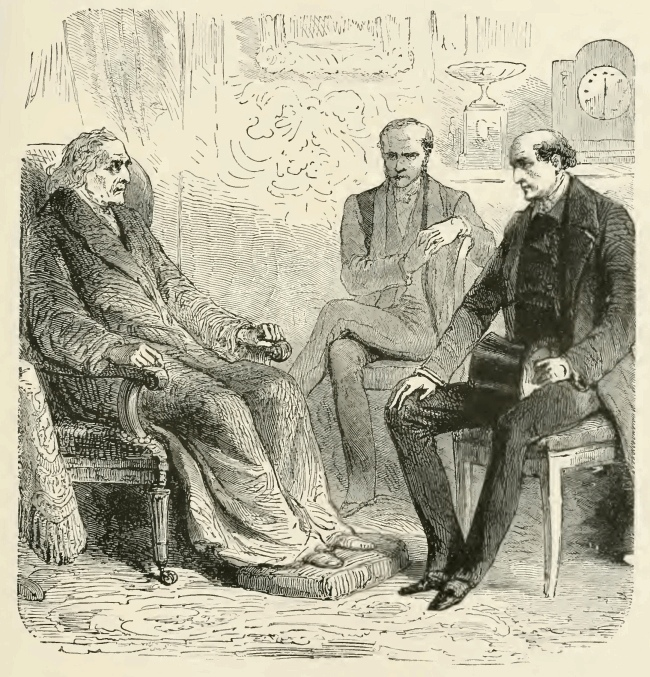
\includegraphics[width=\textwidth]{30175m.jpg}
\end{figure}

“Yes,” looked the invalid, his eye beaming with delight at the ready
interpretation of his meaning.

“What is he going to do?” thought Villefort, whose position demanded
much reserve, but who was longing to know what his father’s intentions
were. He left the room to give orders for another notary to be sent,
but Barrois, who had heard all that passed, had guessed his master’s
wishes, and had already gone to fetch one. The procureur then told his
wife to come up. In the course of a quarter of an hour everyone had
assembled in the chamber of the paralytic; the second notary had also
arrived.

A few words sufficed for a mutual understanding between the two
officers of the law. They read to Noirtier the formal copy of a will,
in order to give him an idea of the terms in which such documents are
generally couched; then, in order to test the capacity of the testator,
the first notary said, turning towards him:

“When an individual makes his will, it is generally in favor or in
prejudice of some person.”

“Yes.”

“Have you an exact idea of the amount of your fortune?”

“Yes.”

“I will name to you several sums which will increase by gradation; you
will stop me when I reach the one representing the amount of your own
possessions?”

“Yes.”

There was a kind of solemnity in this interrogation. Never had the
struggle between mind and matter been more apparent than now, and if it
was not a sublime, it was, at least, a curious spectacle. They had
formed a circle round the invalid; the second notary was sitting at a
table, prepared for writing, and his colleague was standing before the
testator in the act of interrogating him on the subject to which we
have alluded.

“Your fortune exceeds 300,000 francs, does it not?” asked he. Noirtier
made a sign that it did.

“Do you possess 400,000 francs?” inquired the notary. Noirtier’s eye
remained immovable.

“500,000?” The same expression continued.

“600,000—700,000—800,000—900,000?”

Noirtier stopped him at the last-named sum.

“You are then in possession of 900,000 francs?” asked the notary.

“Yes.”

“In landed property?”

“No.”

“In stock?”

“Yes.”

“The stock is in your own hands?”

The look which M. Noirtier cast on Barrois showed that there was
something wanting which he knew where to find. The old servant left the
room, and presently returned, bringing with him a small casket.

“Do you permit us to open this casket?” asked the notary. Noirtier gave
his assent.

They opened it, and found 900,000 francs in bank scrip. The first
notary handed over each note, as he examined it, to his colleague.

The total amount was found to be as M. Noirtier had stated.

“It is all as he has said; it is very evident that the mind still
retains its full force and vigor.” Then, turning towards the paralytic,
he said, “You possess, then, 900,000 francs of capital, which,
according to the manner in which you have invested it, ought to bring
in an income of about 40,000 livres?”

“Yes.”

“To whom do you desire to leave this fortune?”

“Oh!” said Madame de Villefort, “there is not much doubt on that
subject. M. Noirtier tenderly loves his granddaughter, Mademoiselle de
Villefort; it is she who has nursed and tended him for six years, and
has, by her devoted attention, fully secured the affection, I had
almost said the gratitude, of her grandfather, and it is but just that
she should reap the fruit of her devotion.”

The eye of Noirtier clearly showed by its expression that he was not
deceived by the false assent given by Madame de Villefort’s words and
manner to the motives which she supposed him to entertain.

“Is it, then, to Mademoiselle Valentine de Villefort that you leave
these 900,000 francs?” demanded the notary, thinking he had only to
insert this clause, but waiting first for the assent of Noirtier, which
it was necessary should be given before all the witnesses of this
singular scene.

Valentine, when her name was made the subject of discussion, had
stepped back, to escape unpleasant observation; her eyes were cast
down, and she was crying. The old man looked at her for an instant with
an expression of the deepest tenderness, then, turning towards the
notary, he significantly winked his eye in token of dissent.

“What,” said the notary, “do you not intend making Mademoiselle
Valentine de Villefort your residuary legatee?”

“No.”

“You are not making any mistake, are you?” said the notary; “you really
mean to declare that such is not your intention?”

“No,” repeated Noirtier; “No.”

Valentine raised her head, struck dumb with astonishment. It was not so
much the conviction that she was disinherited that caused her grief,
but her total inability to account for the feelings which had provoked
her grandfather to such an act. But Noirtier looked at her with so much
affectionate tenderness that she exclaimed:

“Oh, grandpapa, I see now that it is only your fortune of which you
deprive me; you still leave me the love which I have always enjoyed.”

“Ah, yes, most assuredly,” said the eyes of the paralytic, for he
closed them with an expression which Valentine could not mistake.

“Thank you, thank you,” murmured she. The old man’s declaration that
Valentine was not the destined inheritor of his fortune had excited the
hopes of Madame de Villefort; she gradually approached the invalid, and
said:

“Then, doubtless, dear M. Noirtier, you intend leaving your fortune to
your grandson, Edward de Villefort?”

The winking of the eyes which answered this speech was most decided and
terrible, and expressed a feeling almost amounting to hatred.

“No?” said the notary; “then, perhaps, it is to your son, M. de
Villefort?”

“No.” The two notaries looked at each other in mute astonishment and
inquiry as to what were the real intentions of the testator. Villefort
and his wife both grew red, one from shame, the other from anger.

“What have we all done, then, dear grandpapa?” said Valentine; “you no
longer seem to love any of us?”

The old man’s eyes passed rapidly from Villefort and his wife, and
rested on Valentine with a look of unutterable fondness.

“Well,” said she; “if you love me, grandpapa, try and bring that love
to bear upon your actions at this present moment. You know me well
enough to be quite sure that I have never thought of your fortune;
besides, they say I am already rich in right of my mother—too rich,
even. Explain yourself, then.”

Noirtier fixed his intelligent eyes on Valentine’s hand.

“My hand?” said she.

“Yes.”

“Her hand!” exclaimed everyone.

“Oh, gentlemen, you see it is all useless, and that my father’s mind is
really impaired,” said Villefort.

“Ah,” cried Valentine suddenly, “I understand. It is my marriage you
mean, is it not, dear grandpapa?”

“Yes, yes, yes,” signed the paralytic, casting on Valentine a look of
joyful gratitude for having guessed his meaning.

\begin{figure}[ht]
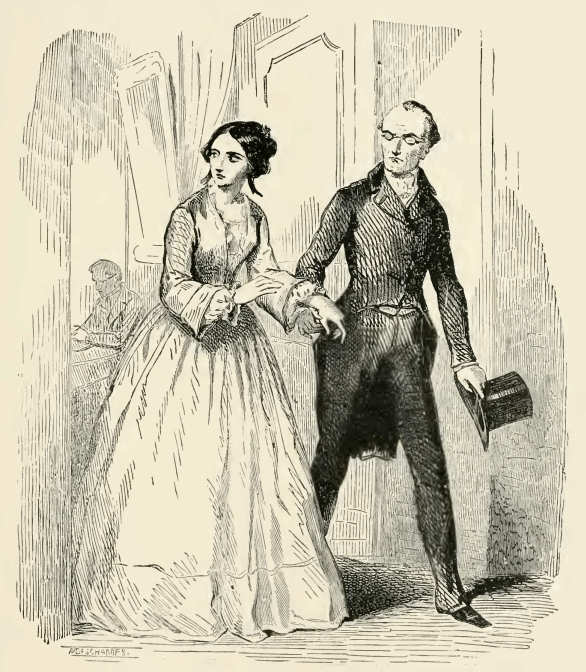
\includegraphics[width=\textwidth]{30179m.jpg}
\end{figure}

“You are angry with us all on account of this marriage, are you not?”

“Yes?”

“Really, this is too absurd,” said Villefort.

“Excuse me, sir,” replied the notary; “on the contrary, the meaning of
M. Noirtier is quite evident to me, and I can quite easily connect the
train of ideas passing in his mind.”

“You do not wish me to marry M. Franz d’Épinay?” observed Valentine.

“I do not wish it,” said the eye of her grandfather.

“And you disinherit your granddaughter,” continued the notary, “because
she has contracted an engagement contrary to your wishes?”

“Yes.”

“So that, but for this marriage, she would have been your heir?”

“Yes.”

There was a profound silence. The two notaries were holding a
consultation as to the best means of proceeding with the affair.
Valentine was looking at her grandfather with a smile of intense
gratitude, and Villefort was biting his lips with vexation, while
Madame de Villefort could not succeed in repressing an inward feeling
of joy, which, in spite of herself, appeared in her whole countenance.

“But,” said Villefort, who was the first to break the silence, “I
consider that I am the best judge of the propriety of the marriage in
question. I am the only person possessing the right to dispose of my
daughter’s hand. It is my wish that she should marry M. Franz
d’Épinay—and she shall marry him.”

Valentine sank weeping into a chair.

“Sir,” said the notary, “how do you intend disposing of your fortune in
case Mademoiselle de Villefort still determines on marrying M. Franz?”
The old man gave no answer.

“You will, of course, dispose of it in some way or other?”

“Yes.”

“In favor of some member of your family?”

“No.”

“Do you intend devoting it to charitable purposes, then?” pursued the
notary.

“Yes.”

“But,” said the notary, “you are aware that the law does not allow a
son to be entirely deprived of his patrimony?”

“Yes.”

“You only intend, then, to dispose of that part of your fortune which
the law allows you to subtract from the inheritance of your son?”
Noirtier made no answer.

“Do you still wish to dispose of all?”

“Yes.”

“But they will contest the will after your death?”

“No.”

“My father knows me,” replied Villefort; “he is quite sure that his
wishes will be held sacred by me; besides, he understands that in my
position I cannot plead against the poor.” The eye of Noirtier beamed
with triumph.

“What do you decide on, sir?” asked the notary of Villefort.

“Nothing, sir; it is a resolution which my father has taken and I know
he never alters his mind. I am quite resigned. These 900,000 francs
will go out of the family in order to enrich some hospital; but it is
ridiculous thus to yield to the caprices of an old man, and I shall,
therefore, act according to my conscience.”

Having said this, Villefort quitted the room with his wife, leaving his
father at liberty to do as he pleased. The same day the will was made,
the witnesses were brought, it was approved by the old man, sealed in
the presence of all and given in charge to M. Deschamps, the family
notary.
